% Chapter Abstract
In this chapter we construct a simple description of \gws as a consequence of \GR. In section~\ref{1:sec:gravitational-radiation} we derive \gws as solutions of the Einstein field equations in a linearised gravity regime under the weak-field approximation. In section~\ref{1:sec:gravitational-wave-detection} we will discuss the ground-based gravitational wave observatories and how gravitational waves will create physical effects which we can measure using these observatories. Finally, in section~\ref{1:sec:modelling_CBC} we will model the gravitational waveform from the primary source of gravitational waves---compact binary coalescences---we see with our detectors. For greater detail on any of these sections, readers are referred to the texts~\cite{Moore_book:2012, Schutz_book:2009, Maggiore_book:2007}.

\section{\label{1:sec:gravitational-radiation}Gravitational radiation}

Gravitational radiation refers to the propagation of perturbations in space-time, predicted by \GR, that manifest as \gws. These waves are generated by the accelerated motion of massive objects and propagate at the speed of light. In this section, we will derive \gws as solutions to the Einstein field equations within the weak-field approximation, where the gravitational field is considered a small perturbation to flat space-time. This approach, known as linearised gravity, allows for a simplified treatment of \gws and provides a foundation for understanding their key properties. We will also discuss the general characteristics of gravitational radiation, such as the polarization and energy carried by \gws.

% Einstein field equations
Einstein's field equations (often referred to as Einstein's equations) are a set of $16$ non-linear independent equations which describe how the gravitational field is generated by matter and can be written very eloquently using \GR notation as
%
\begin{eqnarray}
    G_{\mu\nu} = 8\pi T_{\mu\nu},
    \label{2:eqn:EFE}
\end{eqnarray}
%
where we use natural units, $G = c = 1$.

Einstein's equations relate the curvature of space-time using the Einstein tensor, $G_{\mu\nu}$, to the stress-energy tensor, $T_{\mu\nu}$, which describes the density and flux of matter, energy and momentum at each point in space-time. We note that due to the symmetry of $G_{\mu\nu}$ and $T_{\mu\nu}$ Einstein's equations reduce from $16$ to $10$ independent equations.

\subsection{\label{1:sec:perturbations}Perturbations in space-time}

\Gws are a natural consequence of \GR and we show this by making a number of simplifications to Einstein's equations to reveal valid plane wave solutions to the equations.

We begin in a flat-Minkowski space-time, represented by the space-time metric, $\eta_{\mu\nu}$, and make a \textit{weak} linear perturbation, $h_{\mu\nu}$ due to a gravitational field. In this scenario we can write the metric tensor, $g_{\mu\nu}$, as
%
\begin{equation}
    g_{\mu\nu} = \eta_{\mu\nu} + h_{\mu\nu},
    \label{1:eq:metric_perturbation}
\end{equation}
%
and to ensure our perturbation is small we enforce the condition $|h_{\mu\nu}| \ll 1$. In this regime, we are able to raise and lower indices using the Minkowski metric
%
\begin{equation}
    h^{\mu\nu} = \eta^{\mu\alpha}\eta^{\nu\beta}h_{\alpha\beta}.
    \label{1:eq:raise_lowering_indices}
\end{equation}
%
Terms of $h_{\mu\nu}$ greater than linear-order and negligible and are ignored, this is called taking the \textit{weak-field limit}. This simplification treats the derivation of \gws in a regime where Einstein's equations are linearised, which significantly reduces the complexity of the calculations while still capturing the essential physical behavior of \gws.

We can write the Einstein tensor, $G_{\mu\nu}$, in terms of the Riemann tensor, $R_{\mu\nu}$, the Ricci scalar, $R$, and the metric tensor
%
\begin{align}
    G_{\mu\nu} &= R_{\mu\nu} - \frac{1}{2}g_{\mu\nu}R,
    \label{1:eq:g_munu_riemann}
\end{align}
%
and we can introduce a quantity known at the \textit{trace reverse tensor}
%
\begin{equation}
    \Bar{h}_{\mu\nu} = h_{\mu\nu} - \frac{1}{2} \eta_{\mu\nu}h,
\end{equation}
%
where $h = \eta^{\mu\nu}h_{\mu\nu}$ the trace of the metric perturbation. We call this the 

We can thereby show the linearised Einstein tensor in terms of the linearised Riemann tensor and our trace reverse metric tensor
%
\begin{equation}
    R_{\mu\nu} - \frac{1}{2}g_{\mu\nu}R = \frac{1}{2}\left(\partial^{\sigma}\partial_{\mu}\Bar{h}_{\sigma\nu} - \partial^{\sigma}\partial_{\sigma}\Bar{h}_{\mu\nu} + \partial_{\nu}\partial^{\alpha}\Bar{h}_{\mu\alpha} - \eta_{\mu\nu}\partial^{\alpha}\partial^{\beta}\Bar{h}_{\alpha\beta}\right).
\end{equation}
%
We can then express our fully linearised Einstein field equations as
%
\begin{equation}
    - \Box\Bar{h}_{\mu\nu} + \partial^{\sigma}\partial_{\mu}\Bar{h}_{\sigma\nu}  + \partial_{\nu}\partial^{\alpha}\Bar{h}_{\mu\alpha} - \eta_{\mu\nu}\partial^{\alpha}\partial^{\beta}\Bar{h}_{\alpha\beta} = 16\pi T_{\mu\nu},
    \label{1:eq:linearised_efe}
\end{equation}
%
where $\Box$ is the flat space d'Alembertian operator,
%
\begin{equation}
    \Box = \partial^{\sigma}\partial_{\sigma} = -\frac{\partial^{2}}{dt^{2}} + \frac{\partial^{2}}{dx^{2}} + \frac{\partial^{2}}{dy^{2}} + \frac{\partial^{2}}{dz^{2}}.
\end{equation}
%

\subsection{\label{1:sec:gauge-transformations}Gauge transformations}

Inspecting equation~\ref{1:eq:linearised_efe} we can identify the presence of the d'Alembertian operator $\Box$ along with terms involving divergences of $\bar{h}_{\mu\nu}$. Making a gauge transformation into the 
harmonic gauge (or de Donder gauge), will eliminate the divergences
%
\begin{equation}
    \partial^{\nu} \Bar{h}_{\mu\nu} = 0.
    \label{1:eq:divergence_gone}
\end{equation}
%
In the weak-field limit we can make this gauge transformation by applying small coordinate translations to the perturbed spacetime that ensure the metric perturbations remain small,
%
\begin{align}
    x &\rightarrow x^{\prime}, \\
    x^{\prime\mu} &= x^{\mu} + \xi^{\mu}(x),
    \label{1:eq:gauge_transform}
\end{align}
%
where the metric in the new coordinate system is
%
\begin{equation}
    g^{\prime}_{\mu\nu} = \eta_{\mu\nu} + \bar{h}^{\prime}_{\mu\nu},
    \label{1:eq:gauge_metric}
\end{equation}
%
and remains valid as long as the weak-field approximation still holds in the new coordinates $|h^{\prime}_{\mu\nu}| \ll 1$.

We have chosen a coordinate system where equation~\ref{1:eq:divergence_gone} is satisfied and in this gauge, the Einstein field equations simplify to
%
\begin{equation}
    \Box \Bar{h}_{\mu\nu} = -16 \pi T^{\mu\nu}
    \label{1:eq:lorentz_gauge_efe}
\end{equation}
%

\subsection{\label{1:sec:gw_in_vacuum}Gravitational waves in a vacuum}

In the weak-field approximation, where we are far from any sources of mass or energy ($T_{\mu\nu} = 0$), equation~\ref{1:eq:lorentz_gauge_efe} simplifies to
%
\begin{equation}
    \Box \Bar{h}_{\mu\nu} = 0,
\end{equation}
%
which is the wave equation and has plane wave solutions of $\Bar{h}_{\mu\nu}$,
%
\begin{equation}
    \Bar{h}_{\mu\nu} = A_{\mu\nu} {\rm e}^{i(k_\alpha x^\alpha)},
\end{equation}
%
indicating the wave nature of gravitational perturbations. $A_{\mu\nu}$ is the amplitude tensor and $k_\alpha = (-\omega, \textbf{k})$, the wave vector that satisfies
%
\begin{equation}
    k^{\alpha} k_{\alpha} = 0 = -\omega^{2} + |\vec{k}|^{2}.
    \label{2:eq:wave_vector_trace}
\end{equation}
%
Equation~\ref{2:eq:wave_vector_trace} tells us that $\omega^{2} = |k|^{2}$ meaning the speed of gravity $v = \omega / |k_{i}| = 1$: \gws travel at the speed of light. 

\subsection{\label{}The transeverse-traceless gauge}

We now have solutions to the Einstein field equations which are of the form of plane waves. $\bar{h}_{\mu\nu}$ is a tensor which contains $10$ independent components (as a symmetric tensor in $4$-dimensional space-time) with redundancy between them. We can express another set of gauge transformations to reduce this to a tensor with only $4$ components and $2$ degrees of freedom.

First, we apply the gauge condition stated in equation~\ref{1:eq:divergence_gone}
%
\begin{align}
    0 &= k^{\mu} A_{\mu\nu},
\end{align}
%
this implies that \gws are \textit{transverse}. This removes the components of $\bar{h}_{\mu\nu}$ that are parallel to the direction of propagation of the \gw, $\bar{h}_{0i} = 0$\footnote{Roman letter indices represent spatial dimensions ($x$, $y$, $z$).}. For instance, a \gw travelling in the $z$-direction will have purely spatial components in the $x$ and $y$ directions.

Second, we require $\bar{h}^{\mu}_{\mu} = 0$, the trace of the \gw vanishes. This removes the possibility of a volume change in space-time due to \gwadj transmission. We say that our \gws are now \textit{traceless}. This new gauge is called the \textit{transverse-traceless} (TT) gauge.

\subsection{\label{1:sec:gravitational-propagation}Gravitational wave propagation and interaction}

In the TT gauge, we can express the metric perturbation $h^{TT}_{\mu\nu}$ for a \gw propagating in the $z$-direction
%
\begin{equation}
   h^{TT}_{\mu \nu} =
   \begin{pmatrix}
      0 & 0 & 0 & 0 \\
      0 & h_+ & h_\times & 0 \\
      0 & h_\times & -h_+ & 0 \\
      0 & 0 & 0 & 0
   \end{pmatrix}.
   \label{1:eqn:h_TT}
\end{equation}
%
We define the plus and cross polarisations as
%
\begin{equation}
    h_+ = A_+ \cos(\omega t - \omega z + \Phi_{0}),
\end{equation}
%
\begin{equation}
    h_{\times} = A_{\times} \cos(\omega t - \omega z + \Phi_{0}),
\end{equation}
%
where $A_+$ and $A_\times$ are the amplitudes of the two polarisations, and $\Phi_{0}$ is a constant phase offset. We have described the metric perturbation with only two independent components: the plus ($+$) and cross ($\times$) polarisations, representing the two degrees of freedom in gravitational radiation.

% Gravitational Wave Interactions
We consider the effect of a passing \gw on two particles in the $x$-$y$ plane placed at ($x_{1}, y_{1}$) and ($x_{2}$, $y_{2}$). The space-time interval between the two particles can be written
%
\begin{align}
    \Delta s^{2} &= \left(\eta_{\mu\nu} + h^{TT}_{\mu\nu}\right) \Delta x^{\mu} \Delta x^{\nu}, \\
    &= -dt^{2} + \left(1 + h_{+}\right)(x_{1} - x_{2})^{2} \nonumber \\
    &\quad + \left(1 - h_{+}\right)(y_{1} - y_{2})^{2} \nonumber \\
    &\quad + 2h_{\times} (x_{1} - x_{2})(y_{1} - y_{2}).
\end{align}
%
and in the simple case where ($y_{2} - y_{1} = 0$) we can calculate the proper distance between the two particles at an arbitrary time, $t$, as
%
\begin{equation}
    \Delta s \approx \left( 1 + \frac{1}{2} h_{+}\right)(x_{1} - x_{2}).
    \label{1:eq:proper_dist_two_particles}
\end{equation}
%
We can see that the proper distance between the two particles is stretched by the factor $(1 + \frac{1}{2}h_{+})$. It can be shown that the simultaneous motion in the $y$-direction is a squeezing of the proper distances $(1 - \frac{1}{2}h_{+})$. This change in proper distance is called \gwadj ``strain'' and is what we want to measure to directly observe the effects of \gws.

Figure~\ref{1:fig:ring_of_particles} provides a visual representation of how the proper distances in a ring of particles change under the influence of a gravitational wave with pure $+$ or $\times$ polarization.
%
\begin{figure}
   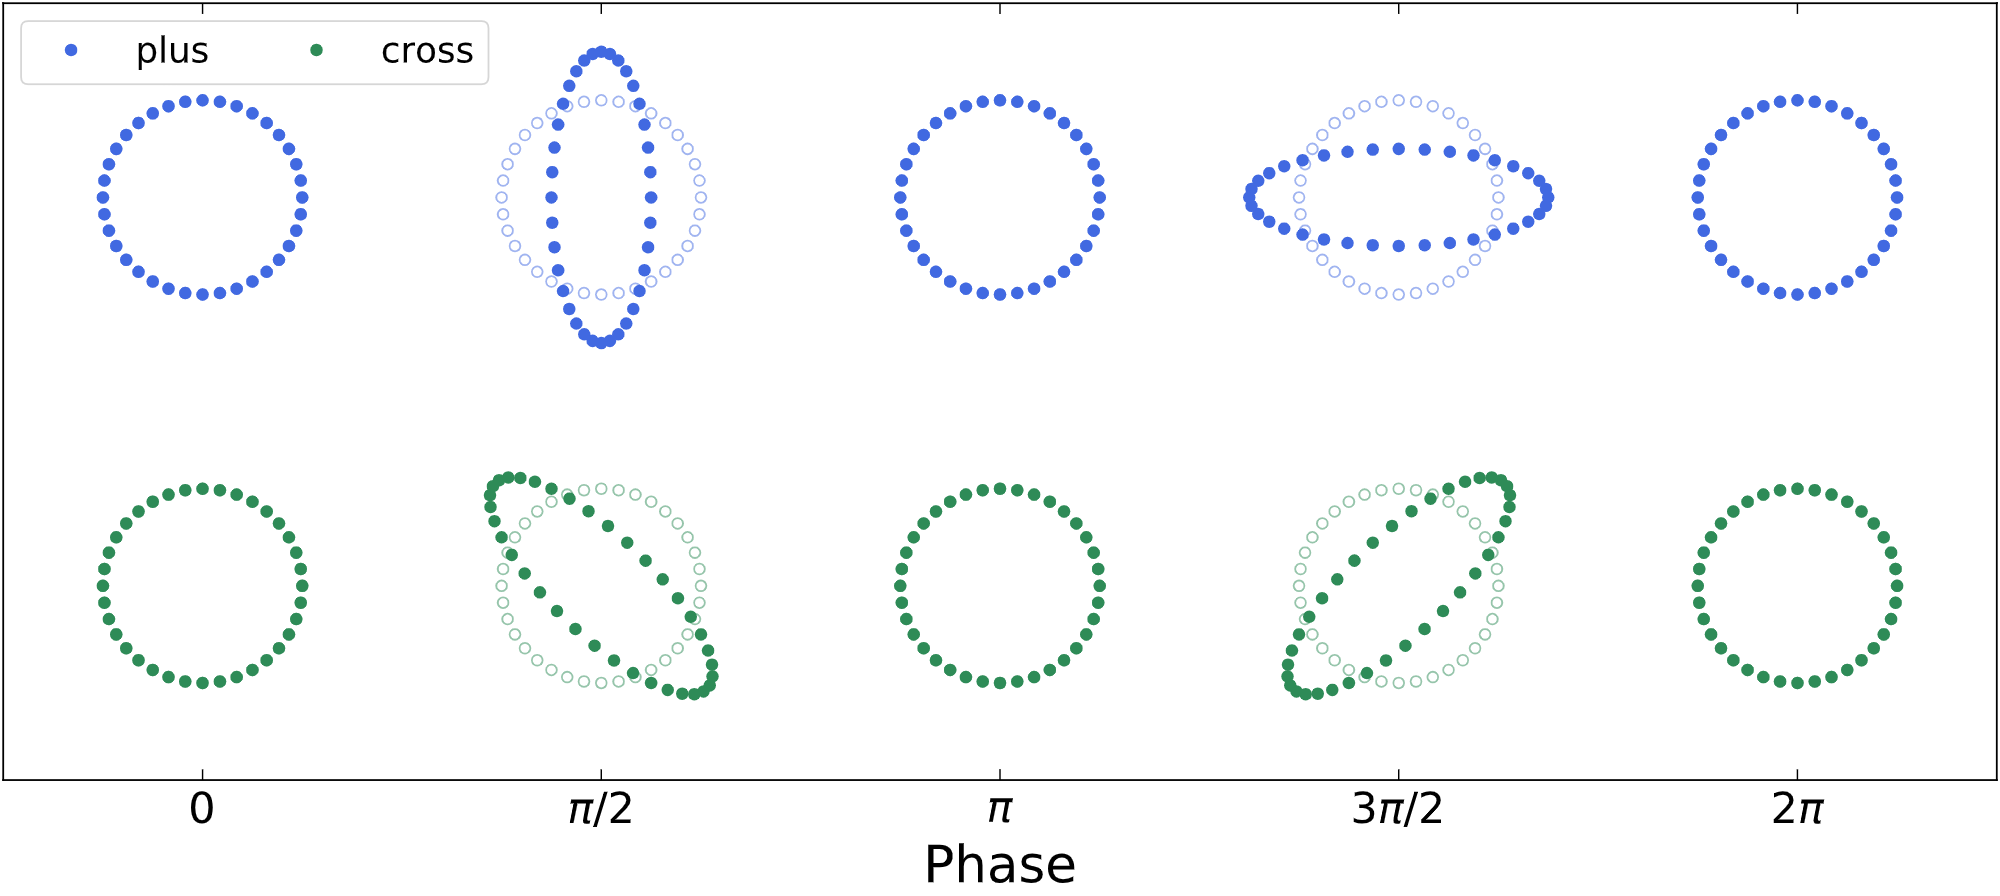
\includegraphics[width=\textwidth]{images/1_general_relativity/polarization.png}
   \caption{The effect of the two polarizations on a ring of test particles~\cite{gw_polarization_plots}.}
   \label{1:fig:ring_of_particles}
\end{figure}
%
It can be seen that the effect of the $\times$ polarisation is the same as the $+$ polarisation but with a $45^{\circ}$ rotation.

\subsection{\label{1:sec:gw-emission}Gravitational wave emission in linearised gravity}

We now return to equation~\ref{1:eq:lorentz_gauge_efe} and reconsider the stress-energy tensor. The solution to the Einstein equations can be obtained using the Green's function
%
\begin{equation}
    \Bar{h}_{\mu\nu}(t, \vec{x}) = 4 \int d^3 x^{\prime} \frac{T_{\mu\nu}\left(t - |\vec{x} - \vec{x}^{\prime}|, \vec{x}^{\prime}\right)}{|\vec{x} - \vec{x}^{\prime}|},
    \label{1:eq:greens_functions}
\end{equation}
%
where the observer is at $\vec{x}$ and the source at $\vec{x}^{\prime}$. The solution can be approximated using the quadrupole formula under two assumptions: the observer is far away $\left(|\vec{x} - \vec{x}^{\prime}| \approx |\vec{x}| = r\right)$ and the source velocity is small compared to the speed of light. 

We expand the stress-energy tensor using a Taylor expansion around the retarded time ($t - r$) and equation~\ref{1:eq:greens_functions} simplifies to
%
\begin{equation}
    \Bar{h}_{\mu\nu}(t, \vec{x}) = \frac{4}{r} \int d^3 x^{\prime} T_{\mu\nu}\left(t - r, \vec{x}^{\prime}\right),
    \label{1:eq:quadrupole_simplification}
\end{equation}
%
in the leading order. We can see that the \gws are dependent on the integral of the stress-energy tensor over a volume containing the source, evaluated at the retarded time.

In the TT gauge, and using the laws of conservation of total energy and momentum, the right-hand side of equation~\ref{1:eq:quadrupole_simplification} can be expressed as
%
\begin{equation}
    \frac{4}{r} \int d^3 x^{\prime} T_{\mu\nu}\left(t - r, \vec{x}^{\prime}\right) = \frac{2}{r}\frac{\partial^{2}}{\partial t^{2}} \int T_{00} x_{\mu} x_{\nu} d^{3} x^{\prime},
\end{equation}
%
where $T_{00} \approx \rho$, the Newtonian mass density. This expression is referred to as the \textit{mass quadrupole moment tensor} of the mass distribution
%
\begin{equation}
    I_{\mu\nu} := \int T_{00} x_{\mu} x_{\nu} d^{3} x^{\prime},
    \label{1:eq:quadrupole_moment_tensor}
\end{equation}
%
and when substituted into equation~\ref{1:eq:quadrupole_simplification}, we obtain the \textit{quadrupole formula}
%
\begin{equation}
    h^{TT}_{\mu\nu} = \frac{2}{r} \ddot{I}_{\mu\nu}(t-r).
    \label{1:eq:quadrupole_formula}
\end{equation}
%
The key properties of this equation are the dependence of gravitational radiation on the second time derivative of the quadrupole moment tensor, indicating that gravitational waves are produced by rapid changes in the quadrupole moment tensor, such as the accelerations of masses and their directional changes during orbital cycles. Additionally, the gravitational wave strain falls off inversely with distance $r$ from the source.

The total power radiated by a source is the \textit{luminosity flux}, and it must equal the energy carried by the gravitational waves, due to the conservation of energy. We can obtain the luminosity flux by integrating the energy flux over a sphere with infinite radius from the source. The total energy loss rate is expressed as
%
\begin{equation}
    \frac{dE}{dt} = -\mathcal{L},
    \label{1:eq:de_dt}
\end{equation}
%
where $\mathcal{L}$ is the gravitational wave luminosity flux. The luminosity flux at a large distance from the source is given by
%
\begin{equation}
    L = \frac{1}{5} \left\langle \dddot{Q}^{jk} \dddot{Q}_{jk} \right\rangle,
    \label{1:eq:luminosity_flux}
\end{equation}
%
where $Q_{jk}(t)$ is the mass quadrupole moment of the source, defined as
%
\begin{equation}
    Q_{jk}(t) = \int \rho(t, x^i) \left( x_j x_k - \frac{1}{3} \delta_{jk} x_l x^l \right) d^3x,
\end{equation}
%
where $\rho$ is the mass density distribution and $\delta_{jk}$ is the Kronecker delta. The angular brackets represent averaging over all directions, and $\dddot{Q}_{jk}$ refers to the third time derivative of the quadrupole moment. This shows that any source with a non-vanishing second derivative of its mass quadrupole moment will emit gravitational waves.

Thus, through the quadrupole formula and gravitational wave luminosity, we see that rapidly accelerating masses with a non-zero quadrupole moment are ideal sources of gravitational radiation.





















\section{\label{1:sec:gravitational-wave-detection}Gravitational wave detection}

% Introduction to Gravitational Wave Detection
Having described the effect of \gws on a ring of particles, we now describe how these principles can be applied to detect \gws on Earth. The first direct detection of \gws was achieved on the 14th September 2015~\cite{GW150914:2016}, made possible by the \gwadj observatories. Currently, the network of operational gravitational wave detectors includes the Advanced LIGO (aLIGO) detectors located in Hanford and Livingston~\cite{aLIGO:2015}; Virgo in Italy~\cite{aVirgo:2015}; KAGRA in Japan~\cite{KAGRA:2021}; and GEO600 in Germany~\cite{GEO600:2002}. While this section will primarily focus on the design and operation of the aLIGO interferometers, the underlying detection principles are similar across all observatories. The configuration and performance of aLIGO are described comprehensively in~\cite{aLIGO:2015}.

\subsection{\label{1:sec:laser_interferometry}Laser interferometry}

% Basic Concept of Laser Interferometry
The physical effect of a passing \gw on a ring of particles (figure~\ref{1:fig:ring_of_particles}) is described as a stretching and squeezing, changing the particles' proper distances depending on the polarisation of the \gw. The \gwadj observatories are Michelsonn interferometers and we can visualise the L-shape of them as experiencing similar effects to the ring of particles. A basic diagram of the LIGO interferometer design can be seen in figure~\ref{1:fig:ifo}.
%
\begin{figure}
    \centering
    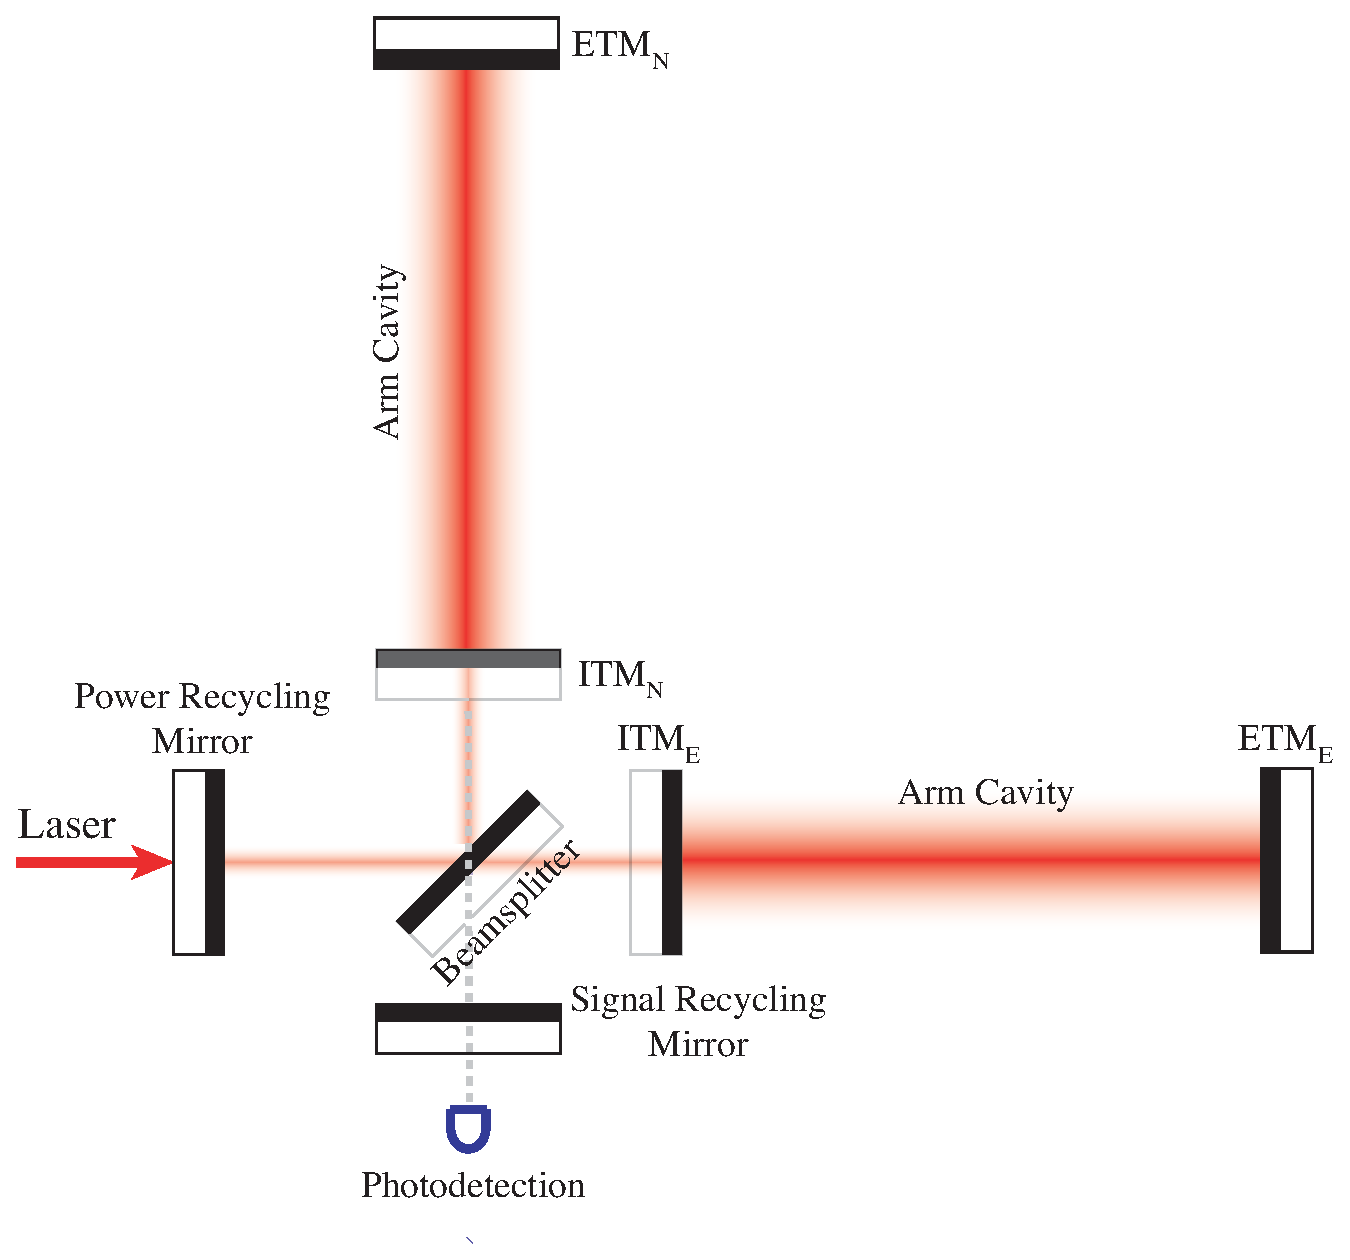
\includegraphics[width=1.0\linewidth]{images/1_general_relativity/gravitational_wave_detection/IFO.eps}
    \caption{Caption taken from~\cite{IFO_diagram:2008}}
    \label{1:fig:ifo}
\end{figure}
%

Half the light from the laser incident on the beam splitter is transmitted to the end test mass to the north (ETM$_{N}$) which we will refer to as the $y$-direction, and half to the end test mass to the east (ETM$_{E}$), $x$-direction. The end test masses are mirrors which reflect the light back toward the beam splitter. When no gravitational wave is present, the length of the $x$ and $y$ arm cavities are equal and the light returning to the beam splitter interferes destructively meaning no light is detected by the photo-detector output of the detector.

% Effect of Gravitational Waves on the Interferometer
Under the presence of a \gw we would expect to see the same stretching and squeezing experienced by the ring of test particles, we express the effects of the \gw in terms of a `strain'. When the difference in arm lengths is greater than 0 there will be non-total destructive interference at the detector output. The passing \gwadj signal is imprinted in this stretching and squeezing motion and this is what we measure using laser interferometry.

% Mathematical Representation of the Spacetime Metric
In the detector's rest frame when a \gw passes through the interferometer the length of the arm cavities is changed. We can calculate the proper distance between the end test mass in the $x$-arm and the beam splitter of the interferometer using equation~\ref{1:eq:proper_dist_two_particles} where the end test mass is at have a particle at $(L, 0, 0)$ and the beam splitter is placed at the origin
%
\begin{equation}
    ds_{x} \approx \left(1 + \frac{1}{2}h_+\right)L,
\end{equation}
%
where $L$ is the length of the detector arm ($4 \, \text{km}$ for advanced LIGO). The proper distance between beam splitter and end test mass in the $y$ arm (position ($0, L, 0)$ will be
%
\begin{equation}
    ds_{y} \approx \left(1 - \frac{1}{2}h_+\right)L,
\end{equation}
%
The strain experiences by the $x$ and $y$ arms is directly related to both the magnitude of the $h_{+}$ \gwadj polarisation and the length of the detector arm. The arm in the $x$-direction will experience a stretching while the $y$ arm will experience a squeezing and vice-versa. 

% Calculating the Length Change in Interferometer Arms
The coupling of motion in both arms leads us to require the use of the differential change in arm length to calculate the \gwadj strain
%
\begin{equation}
    h(t) = \frac{\delta L_1 - \delta L_2}{L},
\end{equation}
%
where $\delta L_{1}$ and $\delta L_{2}$ are the changes in the lengths of the arms and $L$ is the length of the arms under no \gw influence.

We need to generalise our $h(t)$ equation for any \gw of any polarisation. The strain induced in a single arm pointing in the $\mathbf{\vec{n}}$ direction, where $\mathbf{\vec{n}}$ is a unit normal vector, is
%
\begin{equation}
    \frac{\delta L}{L} = \frac{1}{2} h_{ij}n^{i}n^{j}
\end{equation}
%
and the difference in lengths for two interferometer arms is
%
\begin{equation}
    h(t) = \frac{1}{2} h_{ij}n_{1}^{i}n_{1}^{j} - \frac{1}{2} h_{ij}n_{2}^{i}n_{2}^{j},
\end{equation}
%
where crucially $h_{ij}$ is measured in the detector's reference frame. The \gw observed by the detector will not be the same \gw emitted by the source, if we know $h_{ij}$ in the source frame we can transform it into the detector frame using a set of rotations by angles ($\Theta, \Phi, \Psi$).
%
% FIGURE OF THIS ROTATION
%
First, we must define a rotation tensor
%
\begin{equation}
    R^{i}_{j} = 
    \begin{pmatrix}
        \cos\Phi & -\sin\Phi & 0 \\
        \sin\Phi &  \cos\Phi & 0 \\
        0        &  0        & 1
    \end{pmatrix}
    \begin{pmatrix}
        1 & 0 & 0 \\
        0 & \cos\Theta & -\sin\Theta \\
        0 & \sin\Theta & \cos\Theta \\
    \end{pmatrix}
    \begin{pmatrix}
        \cos\Psi & -\sin\Psi & 0 \\
        \sin\Psi &  \cos\Psi & 0 \\
        0        &  0        & 1
    \end{pmatrix}
    \label{1:eq:detector_frame_rotations}
\end{equation}
%
and when transforming the spatial components of $h_{ij}$ using this tensor we can evaluate the detector strain as a function of the $+$ and $\times$ polarisations in the radiation frame and the three angles relating the radiation frame to the detector frame. A detector with arms aligned in the $x$ and $y$ directions will give
%
\begin{equation}
    h(t) = F_{+}(\Theta, \Phi, \Psi)h_{+}(t) + F_{\times}(\Theta, \Phi, \Psi)h_{\times}(t) ,
    \label{1:eq:h_t_linear_combination}
\end{equation}
%
where
%
\begin{equation}
    F_{+}((\Theta, \Phi, \Psi)) = \frac{1}{2}(1 + \cos^{2}(\Theta))\cos2\Phi\cos2\Psi - \cos\Theta\sin2\Phi\sin2\Psi,
\end{equation}
%
\begin{equation}
    F_{\times}((\Theta, \Phi, \Psi)) = -\frac{1}{2}(1 + \cos^{2}(\Theta))\cos2\Phi\cos2\Psi - \cos\Theta\sin2\Phi\sin2\Psi.
\end{equation}
%
Using these rotations we can obtain the antenna response oft he detector to the $+$ and $\times$ polarisations $F_{+}$ and $F_{\times}$ which describe the sensitivity of the detector to \gws at different sky positions. 

% Relating Strain to Gravitational Wave Signal
The induced strain expected from passing gravitational waves is on the order of $\mathcal{O}(10^{-22})$, representing an extraordinarily small distortion in length. The laser light wavelength is approximately $1 \, \text{$\mu$ m}$, therefore, even with arm lengths of order $\mathcal{O}(10^{3})$ strains this small correspond to ${\sim}10^{-13}$ wavelengths of light. This is effectively impossible to measure and we require more advanced interferometer techniques to increasing our possibility of detection.

% Conclusion

\subsection{\label{}Increasing detector sensitivity}

Equation~\ref{1:eq:delta_phi} tells us that the phase difference measured by the detector is propertional to the total arm length of the detector. The advanced LIGO detectors have an arm length of $4 \, \text{km}$ which, while long, are not nearly long enough for a gravitational wave signal to have an appreciable change in length effect. We can effectively increase the arm length of the detectors be making the light travel down the arms multiple times. The Fabry-Perot cavities in the arms of the aLIGO detectors contain an additional mirror on the input test mass (ITM) which face each other and have high reflectivity, allowing only a small fraction of light to transmit through. Not only will the light now continuously build up in power as it reflects many times between these two mirrors but the effect of the light travelling a much greater distance will lead to a greater phase difference between the light in both arms under the presence of a gravitational wave signal.


















\section{\label{1:sec:modelling_CBC}Modelling compact binary coalescences}

The primary sources of \gws seen by Earth-based \gwadj detectors are those from \cbcs. \Cbcs (CBC) are the inspiral and merger of two compact objects (black holes or neutron stars), these two objects have typically been locked into a binary star system their whole lives. The binary system will emit \gws which slowly dissipates the orbital energy of the system. A decreasing orbital energy leads to a decreasing orbital radius which itself leads to a increased orbital velocity and greater acceleration leading to an even greater disspitation of orbital energy---and more energetic \gwadj emission. The orbital radius decays into an eventual merger between the two objects. We have observed three distinct CBC systems: binary black holes (BBH), binary neutron stars (BNS) and neutron star - black hole binaries. 

We describe the \gws emitted by a compact binary merger and the physical effects these would have on \gwadj detectors. First, we need to describe the intrinsic properties of the system which have an effect on the gravitational wave signal being created and the extrinsic, observational parameters which change the signal based on how it is being observed. Next, we derive a gravitational waveform with a very simple binary system of two point-like masses using the Newtonian formalism.

\subsection{\label{1:sec:CBC-parameters}Waveform parameters}

\subsubsection{Intrinsic parameters}
The intrinsic parameters are those which have physical effects on the system and alter how the gravitational wave signal is created.
\begin{itemize}
   \item Primary and secondary component masses, $m_{1}$ and $m_{2}$
   \item Primary and secondary three-dimensional spin vector, $\vec{s_{1}}$ and $\vec{s_{2}}$
\end{itemize}
Here, the subscript $_1$ refers to the more massive object in the binary system, and $_2$ to the less massive one.

\subsubsection{Extrinsic parameters}
The extrinsic parameters affect how the gravitational wave signal is observed.
\begin{itemize}
   \item Right ascension of the source location, $\alpha$ 
   \item Declination of the source location, $\delta$
   \item Luminosity distance to the source$r$, 
   \item Inclination angle between the line of sight and the orbital angular momentum of the binary, $\iota$
   \item Polarization angle of the gravitational wave, $\psi$
   \item Time of coalescence, $t_{c}$
   \item Coalescence phase, $\phi_{c}$ 
\end{itemize}

While these are the fundamental parameters that define a CBC waveform, additional parameters may describe other physical effects. These include tidal deformations, eccentricity, the neutron star equation of state, or potential deviations from \GR. However, in this work, we will ignore these additional effects and focus on the parameters listed above.

\subsection{\label{}Binary inspiral in Keplerian motion}

We can derive $h_{+}$ and $h_{\times}$ for a binary system modelled as a simple closed circular orbit of two point masses around a shared centre of mass. These two point masses are in the `inspiral' regime, where they are radiating \gws and are not close to merging. We choose a frame of reference where the plane of the binary is in the $x$-$y$ direction and the binary is situation at a distance $r$ from the origin.

We obtain the orbital velocity in Kepler's laws of planetary motion by equating the Newtonian gravitational force and the orbital centripetal force
%
\begin{align}
    \frac{m_{1} m_{2}}{a^{2}} = \frac{\mu v^{2}}{a}, \\
    v = \sqrt{\frac{m_{1} + m_{2}}{a}},
\end{align}
%
where $m_{1}$ and $m_{2}$ are the masses of the objects, $\mu$ is the reduced mass of the system and $a$ is the distance between the two objects.
%
We obtain the orbital frequency using $\omega = v/a$,
%
\begin{equation}
    \omega_{orbit} = \sqrt{\frac{m_{1} + m_{2}}{a^{3}}},
    \label{1:eq:omega_orbit}
\end{equation}
%
and relate it to the rate of change in the orbital phase
%
\begin{equation}
    \omega_{orbit} = \frac{d \Phi_{orbit}}{dt}.
\end{equation}
%
Using the quadrupole formula (equation~\ref{1:eq:quadrupole_formula}) we can derive the metric perturbations caused by this system
%
\begin{equation}
    h_{\mu\nu} = \frac{4}{r} \mu a^{2} \omega^{2}_{orbit}
    \begin{pmatrix}
      0 & 0 & 0 & 0 \\
      0 & -\cos\left(2\omega_{orbit}t\right) & -\sin\left(2\omega_{orbit}t\right) & 0 \\
      0 & -\sin\left(2\omega_{orbit}t\right) & \cos\left(2\omega_{orbit}t\right) & 0 \\
      0 & 0 & 0 & 0
   \end{pmatrix}.
\end{equation}
%
The line of sight between the binary system and the observer is defined by the inclination angle, $\iota$, and when projecting the \gwadj emission in the line of sight we get the waveform polarisations,
%
\begin{equation}
    h_{+}(t) = \frac{4}{r} M\eta v^{2} \left(\frac{1 + \cos^{2}\iota}{2}\right)\cos\left(2\omega_{orbit}t+2\Phi_{c}\right),
\end{equation}
%
\begin{equation}
    h_{\times}(t) = \frac{4}{r} M\eta v^{2} \left(\frac{\cos\iota}{2}\right)\sin\left(2\omega_{orbit}t+2\Phi_{c}\right),
\end{equation}
%
where $\eta = \frac{m_{1}m_{2}}{(m_{1} + m_{2})^{2}}$ is the symmetric mass ratio and $\Phi_{c}$ is the coalescence phase of the system. A key observation from these equations are the frequency of the \gws being twice that of the binary orbital frequency.

We have an embedded assumption that the separation distance of the two objects will remain constant. We know that the radiation of \gws will decrease the orbit of the binary system therefore, solving equations~\ref{1:eq:de_dt} and~\ref{1:eq:luminosity_flux} we can find the power radiated by the binary system. The energy loss will increase the binary orbital frequency, from this we can calculate the change in phase and amplitude as a function of time.

In the two point source example we relate the orbital velocity, $\omega_{orbit}$ to the particle separation, $a$, using equation~\ref{1:eq:omega_orbit} and then when introducing the \textit{chirp mass} ($\mathcal{M}$) of the binary system
%
\begin{equation}
    \mathcal{M} = \frac{(m_{1}m_{2})^{\frac{3}{5}}}{(m_{1} + m_{2})^\frac{1}{5}},
\end{equation}
%
and solving equations~\ref{1:eq:de_dt} and~\ref{1:eq:luminosity_flux} we are able to determine the power radiated by this system as
%
\begin{equation}
    \frac{dE}{dt} = -\frac{32}{5}(\mathcal{M}\omega_{orbit})^\frac{10}{3}.
    \label{1:eq:cbc_eg_de_dt}
\end{equation}
%
The total energy of the system can be written as
%
\begin{align}
    E &= -\frac{m_{1}m_{2}}{2r}, \\
      &=-\frac{1}{2}(\mathcal{M}^{5} \omega^{2}_{orbit})^\frac{1}{8},
      \label{1:eq:total_energy_cbc}
\end{align}
%
and when substituting this into equation~\ref{1:eq:cbc_eg_de_dt} and solving we obtain the orbital frequency as a function of time
%
\begin{align}
    \omega_{orbit}(t) &= \left(-\frac{256}{5}\mathcal{M}^{\frac{5}{3}}(t - t_{0})\right)^{-\frac{3}{8}}, \\
                      &= \frac{1}{8}\left(\frac{\tau}{5}\right)^{-\frac{3}{8}}\mathcal{M}^{-\frac{5}{8}},
    \label{1:eq:omega_orbit_f_of_tau}
\end{align}
%
where $t_{0}$ is the fiducial starting time for integration which is used to map the time to define a new time variable $\tau = t_{c} - t$.


We can integrate equation~\ref{1:eq:omega_orbit_f_of_tau} over time to find the orbital phase of the \gwadj signal
%
\begin{align}
    \Phi(\tau) &= \int^{t}_{t+{0}} \omega_{orbit} dt, \\ 
    &= -2\left(\frac{5G\mathcal{M}}{c^{3}}\right)^{-\frac{5}{8}} \tau^{\frac{5}{8}} + 2\Phi_{c},
\end{align}
%
where $\Phi_{c}$ is the coalescence phase.

Finally, combining the previous equations we have derived
%
\begin{equation}
    h_{+}(\tau) = \frac{1}{r}\left(\frac{G\mathcal{M}}{c^{2}}\right)^{\frac{5}{4}}\left(\frac{5}{c\tau}\right)^{\frac{1}{4}}\left(\frac{1+\cos^{2}\iota}{2}\right)\cos\Phi(\tau),
\end{equation}
%
\begin{equation}
    h_{\times}(\tau) = \frac{1}{r}\left(\frac{G\mathcal{M}}{c^{2}}\right)^{\frac{5}{4}}\left(\frac{5}{c\tau}\right)^{\frac{1}{4}}\cos\iota\sin\Phi(\tau),
\end{equation}
%
the gravitational wave polarisations for a metric perturbation originating from our simple two point particle binary system. From these equations it's easy to show that both the amplitude and frequency of the system will increase rapidly and ``chirp'' as it approaches coalescence, hence the common name of \textit{chirp signal}. Also clear to see is that these gravitational wave signals are dependent only on the chirp mass of the system\footnote{We have chosen to keep $G$ and $c$ as they contribute to the strain value we expect from \gws.}.

\subsection{\label{1:sec:fourier_transform_chirp}Fourier transform of the chirp signal}

In \gwadj analysis, the Fourier transform of a chirp signal is crucial for understanding its frequency domain characteristics. We consider a gravitational waveform given by
%
\begin{equation}
    h(t) = A(t) \cos \Phi(t),
\end{equation}
%
where \( A(t) \) represents the amplitude, and \( \Phi(t) \) is the phase of the signal. To simplify our analysis, we use the \textit{stationary phase approximation}, which is applicable when the amplitude \( A(t) \) varies slowly compared to the phase \( \Phi(t) \). Under this approximation, the Fourier transform of \( h(t) \) is given by
%
\begin{equation}
    \Tilde{h}(f) \simeq \frac{1}{2} A\left(t(f)\right) \left(\frac{dt(f)}{df}\right)^{\frac{1}{2}} {\rm e}^{i \left(2\pi f t(f) - \Phi(f) - \frac{\pi}{4}\right)},
\end{equation}
%
where \( t(f) \) and \( \Phi(f) \) are the time and phase at frequency \( f \). For a chirp signal, these quantities can be expressed as
%
\begin{equation}
    t(f) = t_c - \frac{5}{8\pi}\left(8\pi f\right)^{-\frac{8}{3}} \mathcal{M}^{-\frac{5}{3}},
\end{equation}
%
\begin{equation}
    \Phi(f) = \Phi_c - 2\left(8\pi \mathcal{M} f\right)^{-\frac{5}{3}},
\end{equation}
%
where \( t_c \) is the coalescence time, \( \mathcal{M} \) is the chirp mass, and \( \Phi_c \) is the phase at coalescence.

The Fourier transform of the chirp signal, considering the Newtonian approximation, can be expressed as
%
\begin{equation}
    \Tilde{h}(f) = \sqrt{\frac{5}{24}} \frac{G^2 \mathcal{M}^2}{c^5 d_L} \left(\frac{\pi G \mathcal{M} f}{c^3}\right)^{-\frac{7}{6}} \left(\frac{1 + \cos^2 \iota}{2}\right) {\rm e}^{i \Phi(f; t_c)},
\end{equation}
%
where the phase term \( \Phi(f; t_c) \) is given by
%
\begin{equation}
    \Phi(f; t_c) = \frac{\pi}{4} - \frac{3}{128} \left(\frac{\pi G \mathcal{M} f}{c^3}\right)^{-\frac{5}{3}} - 2\pi f t_c + \Phi_c.
\end{equation}
%
Here, \( d_L \) denotes the luminosity distance to the source, and \( \iota \) is the inclination angle of the orbital plane with respect to the line of sight. This expression provides a compact representation of the chirp signal's frequency domain characteristics, essential for gravitational wave data analysis and signal detection.

\subsection{\label{1:sec:post_newtonian_treatment}Post-Newtonian approximation}

The post-Newtonian (PN) expansion technique is used to refine gravitational waveforms by incorporating relativistic effects beyond the leading-order Newtonian approximation, improving the accuracy of gravitational waveforms by accounting for corrections due to \GR.

The PN expansion is performed by expanding in powers of \( v/c \), where \( v \) is the velocity of the orbiting bodies. The waveform is expressed as a series where each term represents a higher-order correction. For a compact binary coalescence, the waveform can be written as
%
\begin{equation}
    h(t) = h_{\text{Newtonian}}(t) + h_{\text{1PN}}(t) + h_{\text{2PN}}(t) + \cdots,
\end{equation}
%
where \( h_{\text{Newtonian}}(t) \) is the leading-order Newtonian term, and \( h_{\text{1PN}}(t) \) and \( h_{\text{2PN}}(t) \) represent the first and second-order PN corrections, respectively.

The first-order PN correction incorporates terms proportional to \( v/c \). The phase of the waveform is modified by including terms that account for relativistic effects on the inspiral dynamics. For instance, the phase term in the Fourier domain becomes
%
\begin{equation}
    \Phi(f) = \Phi_{\text{Newtonian}}(f) + \Phi_{\text{1PN}}(f),
\end{equation}
%
where \( \Phi_{\text{1PN}}(f) \) is
%
\begin{equation}
    \Phi_{\text{1PN}}(f) = -\frac{3}{128} \left(\frac{\pi G \mathcal{M} f}{c^3}\right)^{-\frac{5}{3}} \left( 1 + \frac{1247}{336} \frac{v^2}{c^2} \right),
\end{equation}
%
where \( \mathcal{M} \) is the chirp mass.

Second-order corrections involve terms proportional to \( (v/c)^2 \). These corrections include higher-order effects such as time-dependent corrections to the phase and amplitude. The second-order phase correction can be expressed as
%
\begin{equation}
    \Phi_{\text{2PN}}(f) = -\frac{3}{128} \left(\frac{\pi G \mathcal{M} f}{c^3}\right)^{-\frac{5}{3}} \left( \frac{3}{4} \left(\frac{v^2}{c^2}\right) - \frac{29}{12} \left(\frac{v^4}{c^4}\right) \right).
\end{equation}
%
These higher-order corrections are particularly important for the analysis of signals in the final stages of coalescence.

\subsection{\label{2:sec:full_waveform}Full Waveform}

The post-Newtonian (PN) formalism is accurate primarily during the inspiral phase of the waveform when the two objects are still distant from each other. However, this formalism does not cover the entire evolution of the system. The system continues to emit gravitational waves throughout the merger and post-merger phases, including the ringdown, where the newly formed object settles into its final shape. The gravitational wave emission peaks during the merger, making it crucial for detecting gravitational waves. The ringdown phase is particularly valuable for testing General Relativity (GR)~\cite{GW150914_TGR:2016, GW170817_TGR:2019, O3_TGR:2021}.

Generating full waveforms requires solving the Einstein field equations using numerical relativity (NR), a process that can take weeks. To efficiently model the entire evolution of the waveform---comprising the inspiral, merger, and ringdown (IMR) phases (see Figure~\ref{1:fig:IMR})---waveform families use a combination of NR waveforms and analytical or semi-analytical approximations. This approach balances accuracy with computational efficiency. The following subsections briefly describe these waveform models.

\begin{figure}
    \centering
    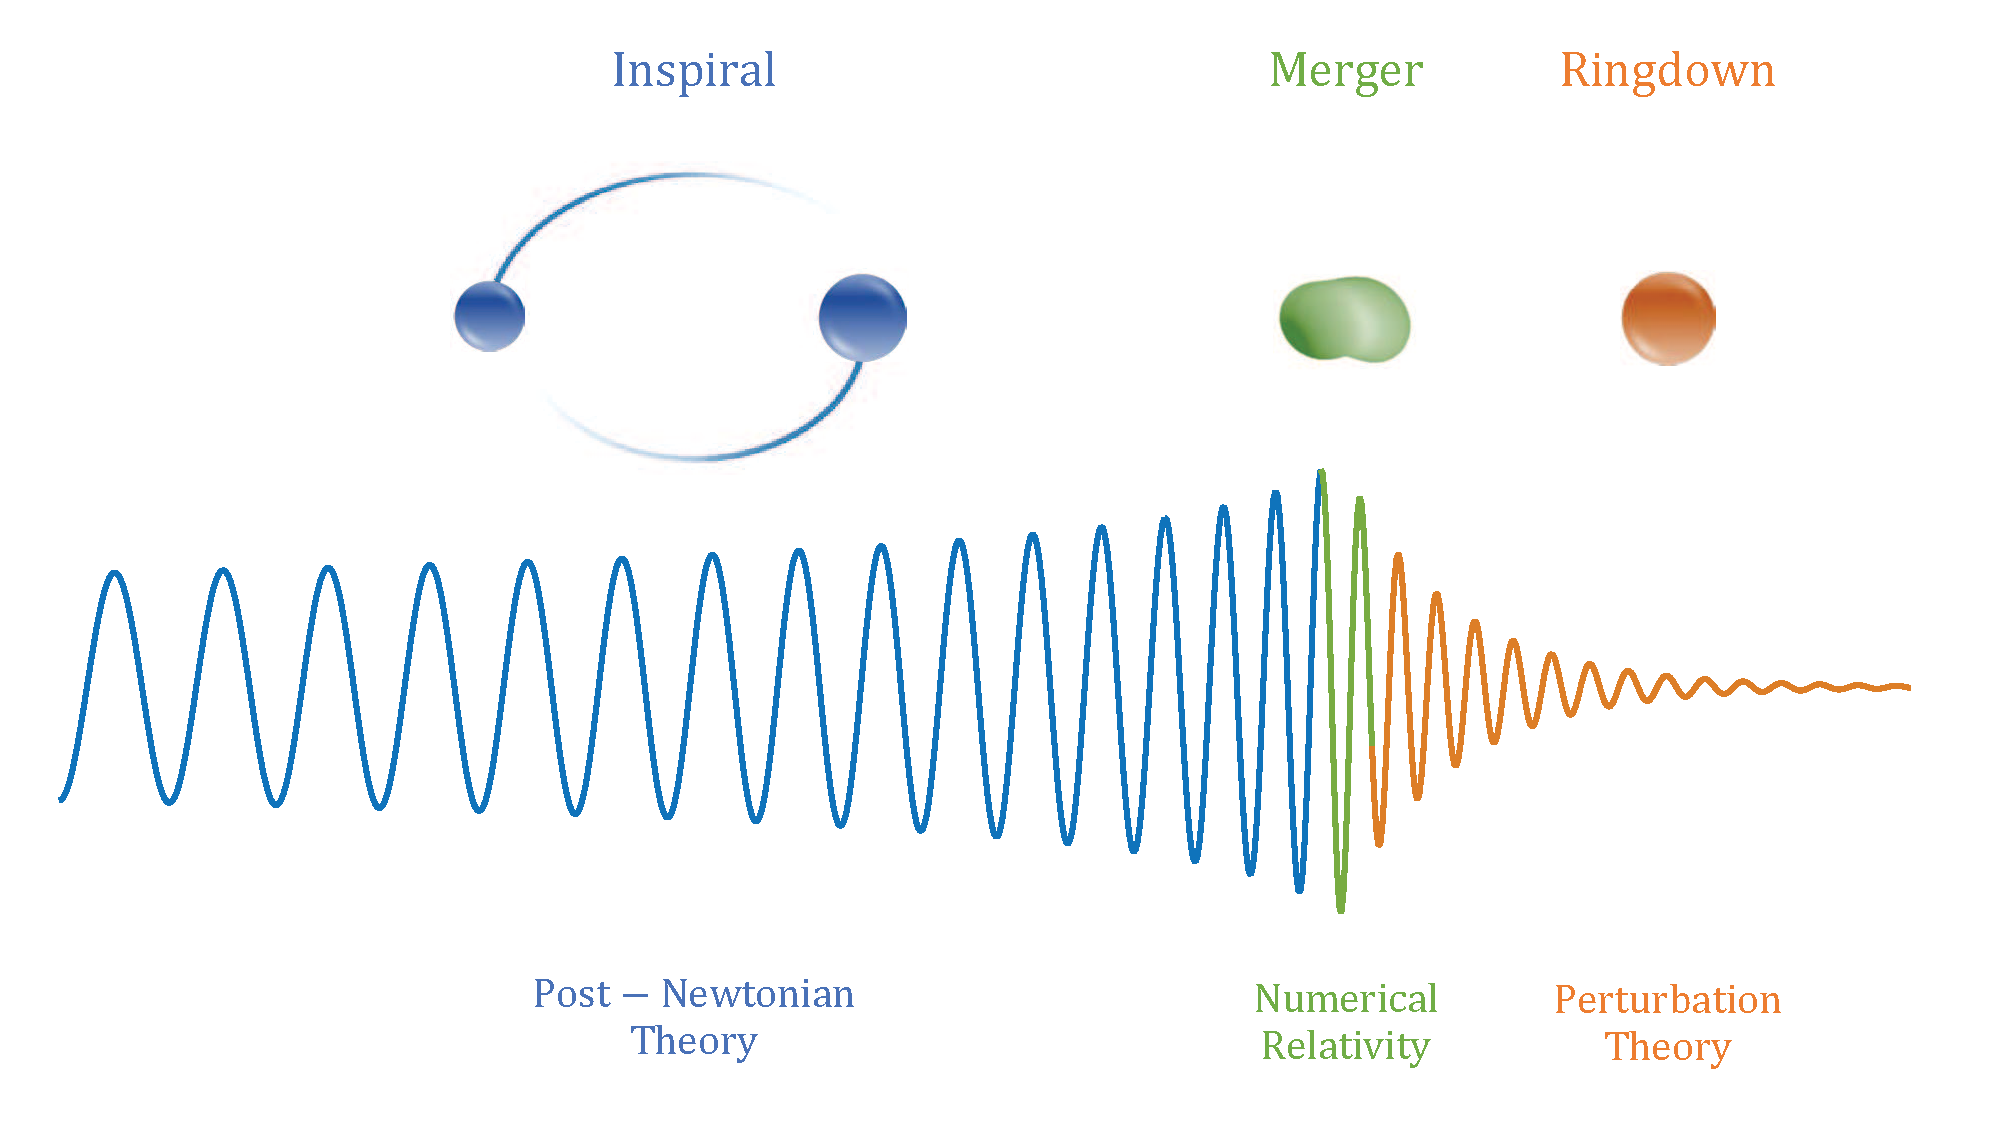
\includegraphics[width=1.0\linewidth]{images/1_general_relativity/modelling_cbc/IMR.pdf}
    \caption{The evolution of a compact binary merger is illustrated through three distinct phases. The inspiral phase involves the two compact objects orbiting each other, with the orbit decaying as they emit gravitational waves. This phase is modeled using post-Newtonian theory. The merger phase occurs when the objects' orbit shrinks sufficiently for them to merge into a new compact object, modeled using numerical relativity. The ringdown phase represents the newly formed object's vibration as it settles into its final shape, modeled using perturbation theory. This image is adapted from~\cite{IMR_plot:2016}.}
    \label{1:fig:IMR}
\end{figure}

\subsubsection{Effective-One-Body (EOB)}

The Effective-One-Body (EOB) model~\cite{EOB_1:1998} simplifies the binary system by transforming it into an equivalent single test particle moving in an external gravitational field, which can be described by a Hamiltonian~\cite{EOB_1:1998, EOB_2:2000, EOB_3:2000, EOB_4:2001}. This Hamiltonian includes both leading-order Newtonian terms and higher-order post-Newtonian corrections~\cite{EOB_5:2008}.

EOB models tuned to numerical relativity (NR) data are known as ``EOBNR'' models~\cite{EOB_6:2007}. Some of these models, such as \verb|SEOBNRv5|~\cite{SEOBNRv5:2023tna}, also incorporate the effects of anti-aligned spins. Further enhancements allow for precession effects and higher-order modes of gravitational wave emission, as seen in the state-of-the-art model \verb|SEOBNRv5_PHM|~\cite{SEOBNRv5_PHM-Buades:2023ehm}, which represents the most advanced waveform model as of this thesis.

\subsubsection{Phenomenological Models}

Phenomenological models, often abbreviated as Phenom, use a phenomenological ansatz calibrated with NR simulations to produce full waveforms. These models are fully analytical and can generate both Fourier domain and time domain waveforms~\cite{IMR_1:2007, IMR_2:2020}. The ability to create waveforms directly in the Fourier domain is highly desirable for analyses that require generating millions of waveforms, such as offline searches or parameter estimation.

Phenom models that cover the inspiral, merger, and ringdown phases are prefixed with \verb|IMRPhenom|~\cite{IMRPhenomD:2009}. The state-of-the-art model in this category is \verb|IMRPhenomXPHM|~\cite{IMRPhenomXPHM:2020}, which can accurately model anti-aligned spins, precessing binaries (\verb|P|), higher-order modes (\verb|HM|), and extreme mass ratios (\verb|X|).

\subsubsection{Surrogate Models}

Surrogate models create waveforms by interpolating from NR simulations~\cite{Surr_1:2019, Surr_2:2022}. These models, such as \verb|NRSur7dq4|~\cite{NRSur7dq4:2019}, provide greater accuracy than earlier models but are limited by the parameter regions covered by the NR simulations used for interpolation. The current leading surrogate model, \verb|NRSur7dq4|, is valid up to a mass ratio of four.
